% =============================================================================
% Autore originale: Fabio Tempera
% Licenza: MIT (vedere LICENSE nel medesimo direttorio)
%
% DOCUMENTO
%   Richiesta di sostegno per la diffusione della rete TESS-4C, da inviare a
%   fondazioni ed enti finanziatori pubblici o privati. Il budget copre il solo
%   costo degli strumenti, nello scenario di 10 stazioni.
%
% COMPILAZIONE
%   pdflatex fondazioni.tex  (due passate per i riferimenti a Figure e Tabelle)
%   Classe report, pacchetti in packages.sty. Non usare Markdown.
% =============================================================================

\documentclass[11pt,a4paper]{report}

\usepackage{packages}

\definecolor{nightblue}{RGB}{22,38,58}
\definecolor{steel}{RGB}{80,100,120}
\definecolor{linegray}{RGB}{200,200,200}

\renewcommand{\thesection}{\arabic{section}}
\renewcommand{\thefigure}{\arabic{figure}}
\renewcommand{\thetable}{\arabic{table}}
\setcounter{secnumdepth}{0}

\titleformat{\section}
  {\normalfont\Large\bfseries\color{nightblue}}
  {\thesection}{0.6em}{}
\titleformat{\subsection}
  {\normalfont\large\bfseries\color{nightblue}}
  {\thesubsection}{0.6em}{}
\titlespacing{\section}{0pt}{1.4em}{0.6em}
\titlespacing{\subsection}{0pt}{1.1em}{0.4em}

\pagestyle{fancy}
\fancyhf{}
\renewcommand{\headrulewidth}{0.4pt}
\renewcommand{\headrule}{\hbox to\headwidth{\color{linegray}\leaders\hrule height \headrulewidth\hfill}}
\fancyhead[L]{\small\color{steel} CieloBuio OdV}
\fancyhead[R]{\small\color{steel} Richiesta di sostegno, rete TESS-4C}
\fancyfoot[C]{\small\color{steel}\thepage}

\hypersetup{
  colorlinks=true,
  linkcolor=nightblue,
  urlcolor=nightblue,
  citecolor=nightblue,
  pdftitle={Richiesta di sostegno. Rete TESS-4C},
  pdfauthor={Fabio Tempera}
}

\setlist[itemize]{leftmargin=1.4em, itemsep=0.25em, topsep=0.3em}
\setlist[enumerate]{leftmargin=1.6em, itemsep=0.25em, topsep=0.3em}

\newcommand{\infobox}[1]{%

  \begin{center}

  \renewcommand{\arraystretch}{1.5}

  \begin{tabularx}{\linewidth}{X}
    \arrayrulecolor{linegray}
    \toprule
    #1 \\
    \bottomrule
  \end{tabularx}

  \end{center}

}

\begin{document}

\begin{center}

{\LARGE\bfseries\color{nightblue} Una rete di stazioni per il monitoraggio del cielo notturno\par}

\vspace{0.2cm}

{\large Richiesta di sostegno per la diffusione della rete TESS-4C\par}

\vspace{0.1cm}

{\small CieloBuio OdV, progetto rete TESS-4C\par}

{\small Documento per fondazioni ed enti finanziatori}

\end{center}

\section*{Sintesi}

\infobox{%
\textit{In sintesi}: il progetto prevede l'installazione di 10 stazioni di misura della brillanza del cielo notturno presso enti selezionati su base volontaria, con un costo degli strumenti da 5.500 a 6.500 EUR. Gli strumenti restano di proprietà di CieloBuio OdV e sono concessi in comodato gratuito agli enti ospitanti. I dati confluiscono in una rete aperta e in un cruscotto pubblico.
}

\section*{Contesto}

L'inquinamento luminoso è l'alterazione della quantità e della distribuzione della luce artificiale nelle ore notturne. Il fenomeno interessa l'osservazione astronomica, l'ecologia, il risparmio energetico e la fruizione del paesaggio notturno come patrimonio culturale. Gli effetti sugli ecosistemi e sugli organismi viventi sono oggetto di ricerca interdisciplinare.

Il passaggio dalle lampade tradizionali ai LED ha aumentato l'efficienza dell'illuminazione, ma ha modificato lo spettro della luce emessa, con una maggiore quota di blu. In molti casi la luce complessiva è aumentata, e le sue conseguenze si estendono ben oltre la sorgente, fino a formare un alone visibile a grande distanza.

Si stima che circa il 99\% della popolazione di Stati Uniti ed Europa viva sotto un cielo inquinato, e che più del 33\% della popolazione mondiale non possa più osservare la Via Lattea (Falchi et al., 2016). In Italia diverse regioni dispongono di norme sul contenimento della luce artificiale. L'applicazione di queste norme richiede però dati oggettivi misurati con continuità, che in molte aree mancano.

Le mappe satellitari restano utili per inquadrare il territorio, ma non misurano la brillanza del cielo a terra. Per monitorare le condizioni locali e l'efficacia degli interventi serve quindi una rete di strumenti collocati sul territorio. La Figura~\ref{fig:contributi} schematizza la brillanza come somma di un contributo naturale e di un contributo artificiale.

\begin{figure}[ht!]
\centering
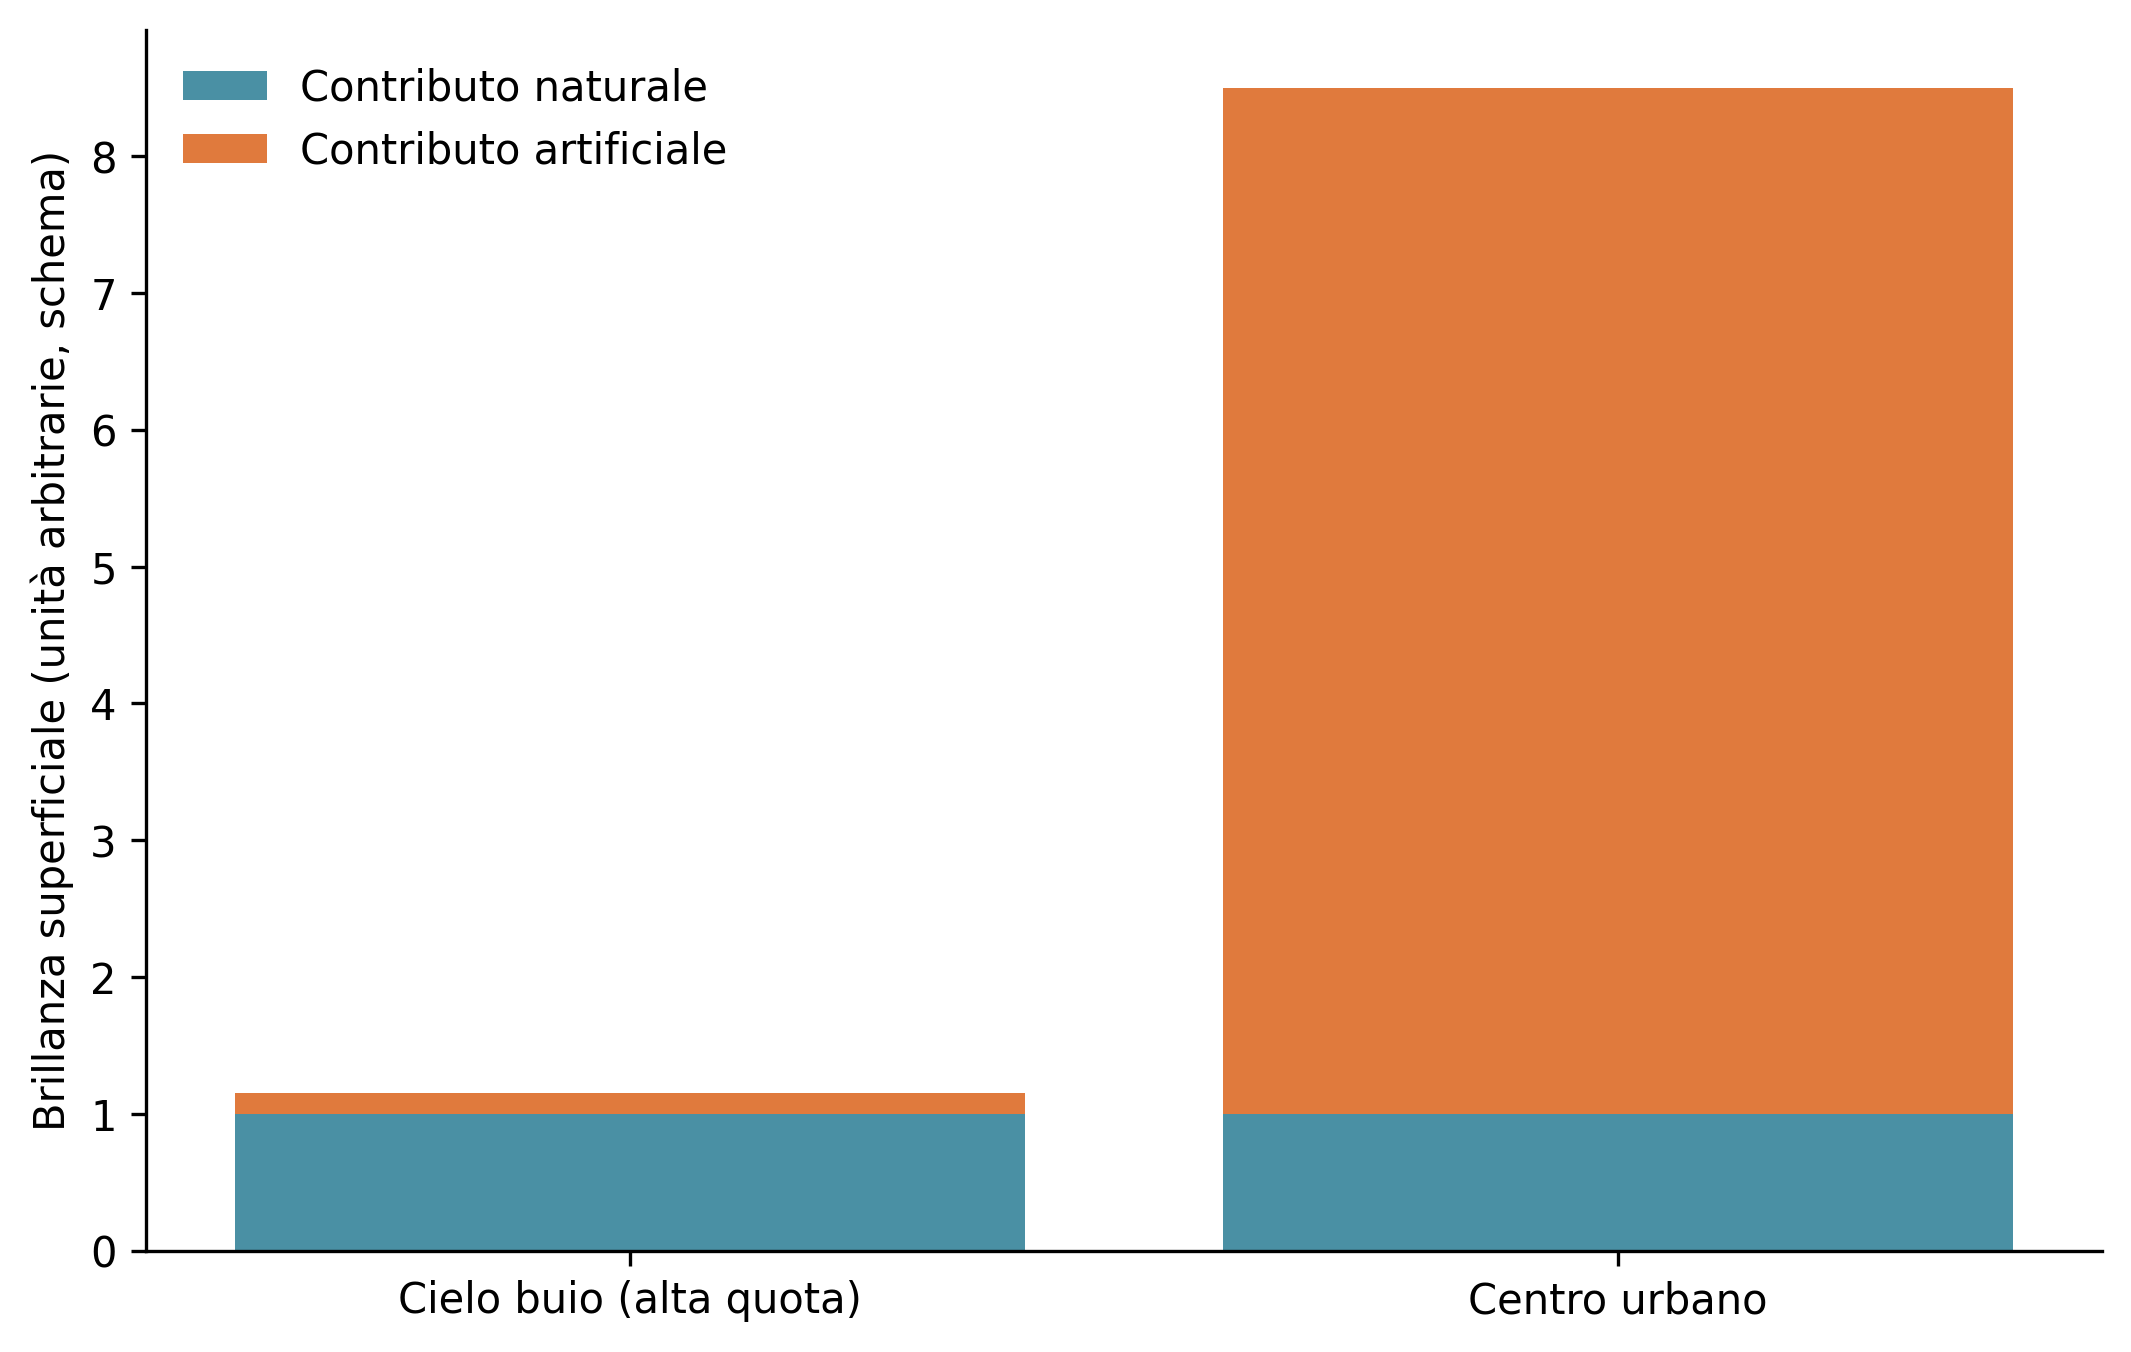
\includegraphics[width=0.85\textwidth]{figures/contributi_brillanza.png}
\caption{Schema della brillanza superficiale come somma di un contributo naturale e di un contributo artificiale. Le altezze delle barre sono illustrative, non misure di un sito specifico.}
\label{fig:contributi}
\end{figure}

\section*{Il progetto TESS-4C}

Il fotometro TESS-4C è l'evoluzione a 4 bande del TESS-W, sviluppato dal gruppo GUAIX dell'Universidad Complutense de Madrid nel progetto europeo STARS4ALL. Lo strumento misura la brillanza superficiale del cielo in 4 canali fotometrici, trasmette i dati via WiFi e richiede un'alimentazione a 5\,V.

La rete non crea un'infrastruttura parallela. Si appoggia alla raccolta dati esistente della rete STARS4ALL, che rende disponibili i dati in formato standard IDA-IAU e in tempo reale sui pannelli Grafana. CieloBuio OdV gestisce un cruscotto di sintesi, con le serie raggruppate per territorio, pensato per la comunicazione pubblica.

\section*{Modello operativo}

Gli strumenti sono acquistati da CieloBuio OdV e restano di sua proprietà. Sono concessi in comodato gratuito a enti selezionati su base volontaria, tra cui:

\begin{itemize}
\item istituti scolastici;
\item enti parco e aree protette;
\item amministrazioni comunali;
\item gruppi astrofili;
\item centri culturali;
\item dipartimenti universitari.
\end{itemize}

La Tabella~\ref{tab:ruoli} descrive la ripartizione dei compiti tra i soggetti coinvolti.

\begin{table}[ht!]

\centering
\renewcommand{\arraystretch}{1.5}

\begin{tabularx}{\linewidth}{@{}l X@{}}
\toprule
Soggetto & Responsabilità \\
\midrule
CieloBuio OdV & acquisto e comodato degli strumenti, coordinamento della rete, cruscotto di sintesi e supporto alla configurazione \\
Ente ospitante & scelta del punto di installazione, affidamento dell'installazione a un tecnico, connessione e cura della stazione \\
Rete STARS4ALL & raccolta dati, formato standard e pannelli in tempo reale \\
\bottomrule
\end{tabularx}

\caption{Ripartizione dei compiti tra CieloBuio OdV, enti ospitanti e rete STARS4ALL.}
\label{tab:ruoli}
\end{table}

Il punto di installazione deve avere zenit libero, assenza di luce artificiale diretta, alimentazione a 5\,V e copertura WiFi verso un router che inoltri i dati. La verifica va fatta in situ, di notte, prima del fissaggio definitivo. CieloBuio OdV fornisce indicazioni, un sopralluogo ove possibile e il supporto a distanza per la configurazione.

\section*{Piano di intervento}

Il piano si articola in 3 fasi, da calibrare in base alle manifestazioni di interesse ricevute.

\begin{enumerate}
\item Raccolta delle manifestazioni di interesse presso gruppi, scuole, enti e amministrazioni, con incontri conoscitivi dedicati.
\item Selezione dei siti in base all'idoneità del punto di installazione e alla disponibilità di un referente locale.
\item Acquisto, installazione, attivazione nella rete e pubblicazione dei dati sul cruscotto pubblico.
\end{enumerate}

\section*{Budget}

La Tabella~\ref{tab:budget} riporta il costo degli strumenti per lo scenario di 10 stazioni.

\begin{table}[ht!]

\centering
\renewcommand{\arraystretch}{1.5}

\begin{tabularx}{\linewidth}{@{}X c c r@{}}
\toprule
Voce & Quantità & Costo unitario & Importo \\
\midrule
Fotometri TESS-4C & 10 & 550-650 EUR & 5.500-6.500 EUR \\
\midrule
Totale & 10 & & 5.500-6.500 EUR \\
\bottomrule
\end{tabularx}

\caption{Costo degli strumenti per lo scenario di 10 stazioni, IVA e spedizione comprese.}
\label{tab:budget}
\end{table}

Il preventivo comprende il solo costo degli strumenti. Le spese di installazione, di manutenzione e di coordinamento non sono incluse nel presente preventivo.

\section*{Risultati attesi}

Al termine della prima fase, ogni stazione attiva produrrà una serie storica di brillanza del cielo notturno, georeferenziata e in formato aperto. Le serie sono utilizzabili per la didattica, la tutela ambientale e la ricerca, e possono sostenere la valutazione delle norme regionali sul contenimento della luce artificiale.

Ogni ente ospitante diventa un riferimento locale per il cielo notturno.

\section*{Prossimi passi}

Per approfondimenti o per un incontro, contattate il referente ai recapiti seguenti.

\vspace{0.2cm}

\noindent Fabio Tempera, CieloBuio OdV

\noindent \url{fabiot2801@gmail.com} \quad$\cdot$\quad WhatsApp 329 883 5142

\end{document}
